%!TEX root=report.tex
\subsection{KMeans}
First off what needed to be identified was the number of clusters. 
Due to the size of the design matrix $X$, (64800,341), and the fact multiple simulated datasets of the same size would be needed to calculate the gap-statistic it was decided to leverage the high performance computing (HPC\footnote{link: http://www.cc.dtu.dk/}) cluster that DTU offers for students and faculty. 
 It should be noted that if such a setup was not available one could have used smaller samples and/or a variant of KMeans using so called "minibatches". \\
5 simulation samples of size (64800,341) was made using a multivariate uniform distribution. The following is the plot of the resulting gap statistic $\pm$ the standard deviation:

\begin{figure}[H]
	\center
	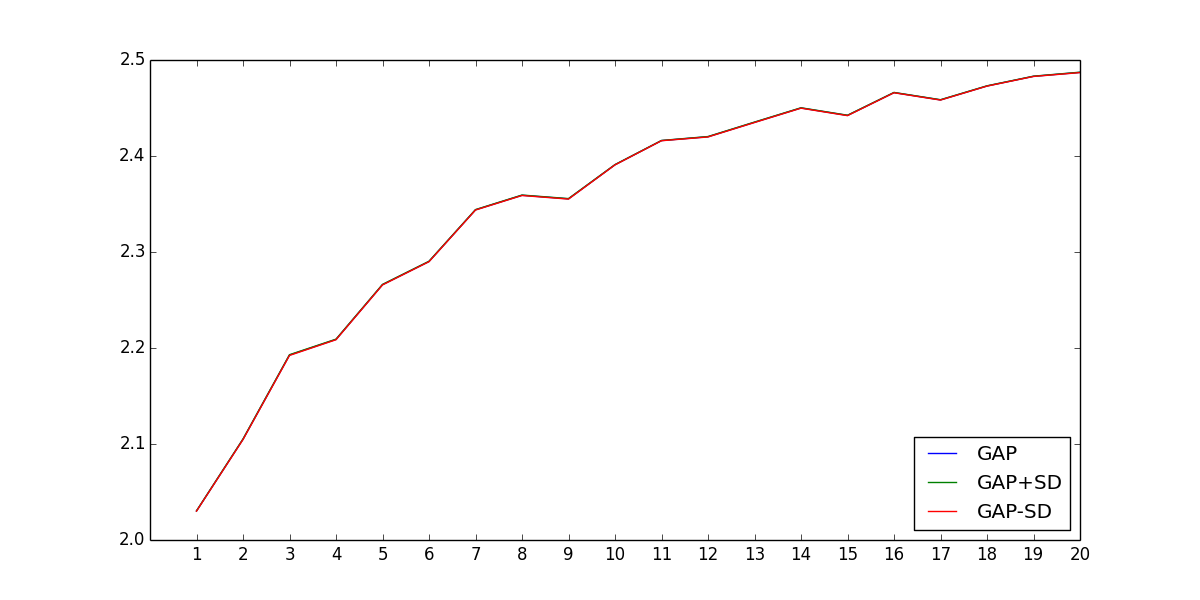
\includegraphics[width=\textwidth]{figures/gap.png}
	\caption{Gap statics and standard deviation. It is not an error that the 3 lines overlap; it is simply caused by the large amount of simulation samples which leads to a very small $W_k$ which in turn causes $SD(Log(W_k)$ to be small ($\approx 10^{-3}$)}
	\label{fig:gap}
\end{figure}

So based on the gap statics plot (or by writing a loop to iterate through values until $gap(k)\ge gap(k+1)-sd(k+1)$) one obtains that 8 clusters should be used. Using 8 cluster, one can color code each cluster in a different color and plot it on the world map, and along side it include af plot of the clusters centroids (color coded in corresponding colors).

\begin{figure}[H]
	\center
	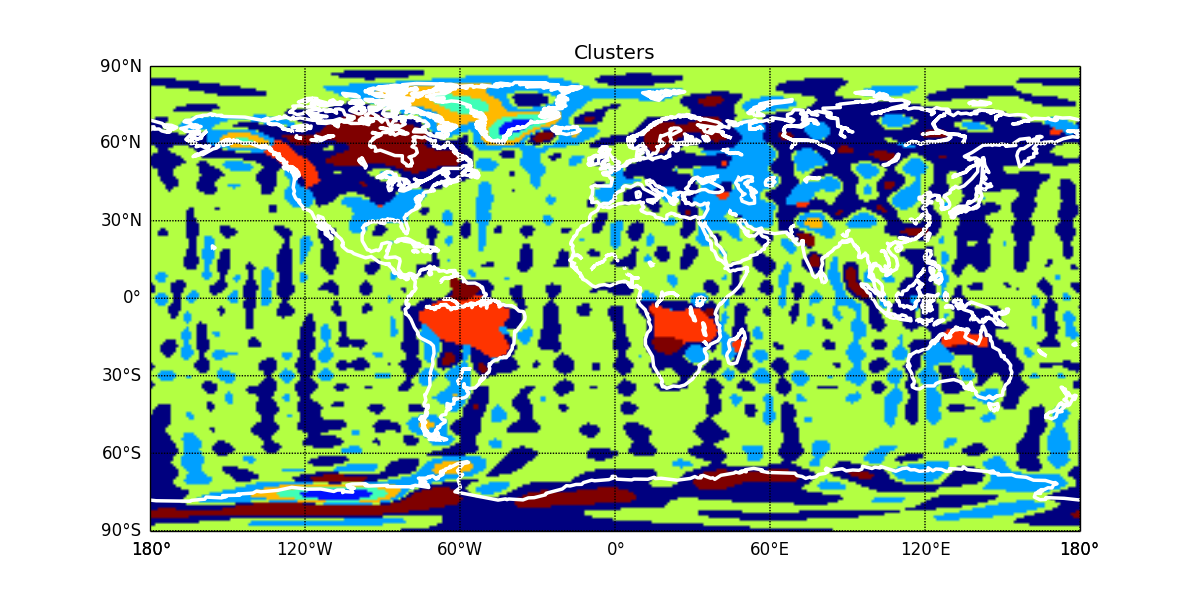
\includegraphics[width=\textwidth]{figures/world_clusters.png}
	\caption{World clusters. See the following plot for the centroids for interpretation}
	\label{fig:world_clusters}
\end{figure}
\begin{figure}[H]
	\center
	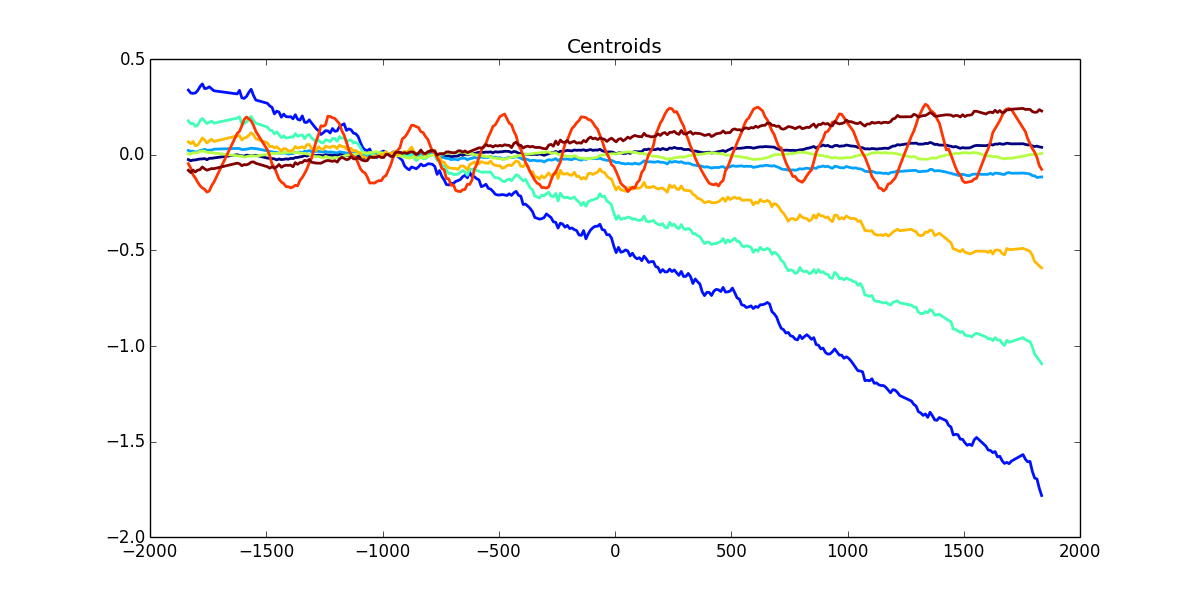
\includegraphics[width=\textwidth]{figures/cluster_centroids.png}
	\caption{Cluster centroids}
	\label{fig:cluster_centroids}
\end{figure}

Comparing the two plot above a few interesting insights are gained
\begin{itemize}
 \item The ocean are primarily green.
\item Some places though the oceans are either dark blue or light blue. Those two centroid appears to be a kind of specific noise that somehow repeats itself across the globe. This might be artifacts from actual noise in the data and or something to do with the spherical kernels that GRACE uses to account for GIA and other phenomena.
\item Dark red areas have a slight mass increase. At the south pole it appears that some of the mass loss at the edge actually moves inward towards the South Pole.
\item  Bright red correlates with extreme and regular seasonality (i.e. rain season in South America)
\item Orange, teal and steel blue correspond with trending mass loss. The most significant locations appear to be located around the tip of the South pole at (60W, 60S) along with Greenland's west and south coast.
\end{itemize}

Finally it should be noted that experiments were made with a higher cluster count. However, as the count increases, as well as making the plot harder to interpret most of the clusters seems to be catching specific noise "trends" in the data. As an example of such an overfit see below.
\begin{figure}[H]
	\center
	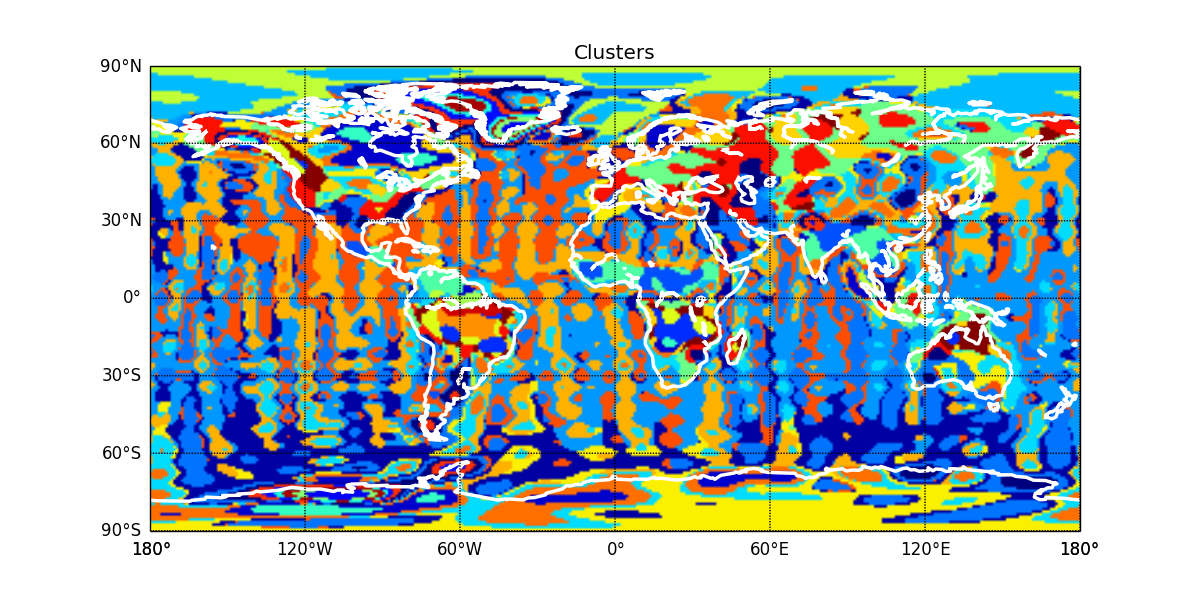
\includegraphics[width=\textwidth]{figures/world_clusters_overfit.png}
	\caption{World clusters overfit. Number of clusters is 30}
	\label{fig:world_clusters}
\end{figure}